%\section{リーフレットについて}
このリーフレットはユーザの木古内町の観光の思い出を1枚の紙面にまとめたものである。リーフレットという形は、ユーザの手間を極力減らすという制約のもと考慮し、紙1枚を両面印刷するだけだが存在感があるという点や、観光の思い出としてその場所のリーフレットやパンフレットを保管する人が一定数いるという背景から決定した。このリーフレットの目的は二つあり、一つは、ユーザが撮影した写真を手がかりにしてその思い出を振り返ること。もう一つは、リーフレットを他の人が見ることによって木古内町の認知度を向上させ、観光客の増加を促進させることである。このリーフレットはキーコ紀行を使って木古内観光を行い、そのあとで7枚の写真を選択することで家庭のAirPrint対応のプリンタを用いて印刷可能で、サイズはA4、巻3つ折りとなっている。表紙には木古内町をイメージさせる、海・山・木古内市街地・新幹線の駅と木古内町の要素が多く詰まった写真に、木古内町観光をした時のものだと分かるように、「みそぎの郷きこない」の文字を表記した。裏表紙や表紙を開いた面には、木古内町の位置や基本的な情報、特産品を記し、木古内町に関する認知度の向上やリピーター増加を狙った。リーフレットをすべて開くと、A4紙全体にユーザが撮影した7枚の写真とその場所に関する説明の文章が印刷された面が見える。この部分がリーフレットの1番の目的で、ここを見ながらユーザに思い出を振り返ってもらうことを想定している。ここに印刷される文章は、アプリ内でもともと設定されているものであるが、よりオリジナリティを求めるユーザは、前述の編集機能を用いて文章を変更することができる。ユーザがその場所でした体験や起こったことに関するエピソードを記せば、その文章と写真がセットで見られることによって思い出の振り返りがより深いものになり、記憶に残るものとなることを期待している。\\\\\\\\\\\\\\

\begin{figure}[htbp]
  \begin{center}
    \begin{tabular}{c}

      % 1
      \begin{minipage}{0.33\hsize}
        \begin{center}
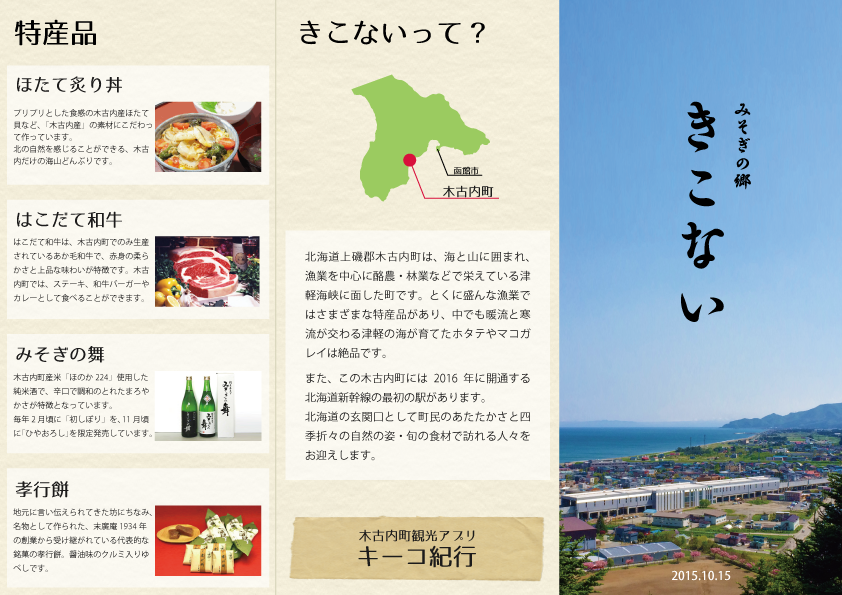
\includegraphics[width=4cm, bb=0 0 842 595]{leaflet_front.png}
          \hspace{1cm} (a)表面。この面の情報は固定。
        \end{center}
      \end{minipage}

      % 2
      \begin{minipage}{0.33\hsize}
        \begin{center}
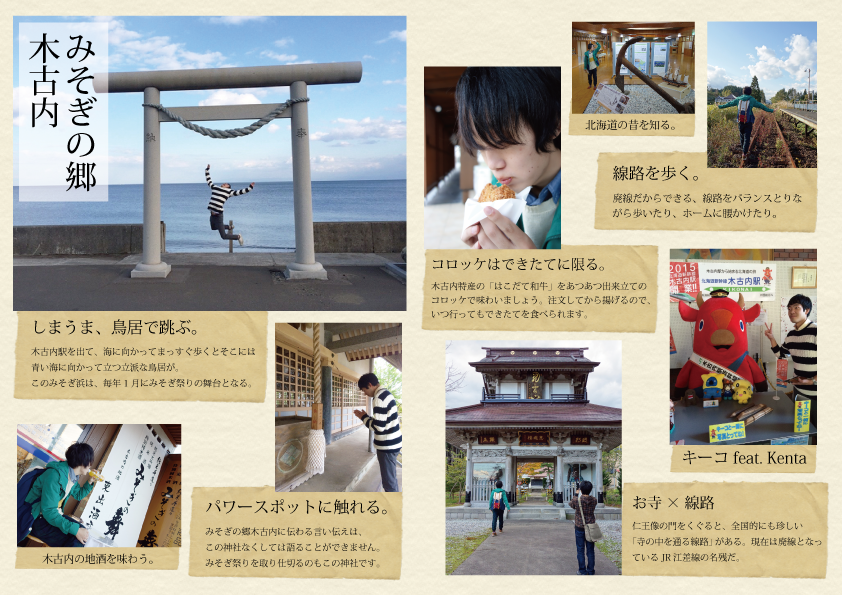
\includegraphics[width=4cm, bb=0 0 842 595]{leaflet_back.png}
          \hspace{1cm} (b)裏面。ユーザの撮影した写真が印刷される。
        \end{center}
      \end{minipage}

    \end{tabular}
    \caption{印刷されるリーフレット}
    \label{fig:lena}
  \end{center}
\end{figure}
\bunseki{細川椋太}